\documentclass{beamer}
\usepackage[utf8]{inputenc}
\usepackage[brazil]{babel}
\usepackage{graphicx}
\usepackage{amsmath}
\usepackage{amsfonts}
\usepackage{amssymb}
\usepackage{tikz}
\usepackage{booktabs}
\usepackage{siunitx}
\usetikzlibrary{shapes, arrows, positioning}

\title{Análise e Projeto de Sistemas de Controle para Reator Químico}
\subtitle{Estudo Comparativo de Técnicas de Controle}
\author{Lucas William Junges}
\institute{Universidade Federal de Santa Catarina \\ Departamento de Engenharia Elétrica e Eletrônica}
\date{\today}

\usetheme{Warsaw}
\usecolortheme{default}

\begin{document}

\begin{frame}
    \titlepage
\end{frame}

\begin{frame}{O Problema: Uma "Fábrica" Química}
    \begin{columns}[T]
        \begin{column}{0.6\textwidth}
            \Huge \textbf{Qual é o nosso objetivo?}
            \vspace{1em}
            
            \Large
            Imagine uma "fábrica" (um reator químico) que produz um líquido valioso (cyclopentenol).
            
            \vspace{1em}
            \alert{Nossa missão:} Manter a \textbf{qualidade} (\(C_b\)) e a \textbf{quantidade} desse líquido sempre perfeitas, de forma automática, mesmo com imprevistos.
            
            \vspace{1em}
            Queremos um "cérebro automático" (controlador) que ajuste o processo sozinho.
            
        \end{column}
        \begin{column}{0.4\textwidth}
            \begin{figure}
                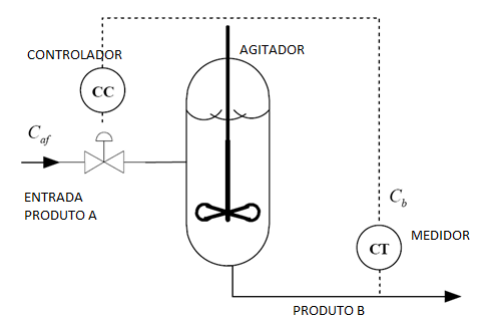
\includegraphics[width=\textwidth]{Imagens/Reator.png}
                \caption{O Reator Químico (CSTR).}
            \end{figure}
        \end{column}
    \end{columns}
\end{frame}

\begin{frame}{A "Receita": Modelagem do Processo}
    \Large A dinâmica do processo é regida por duas reações principais:
    \begin{align*}
        A \xrightarrow{k_1} B \quad & \text{(Produto desejado)} \\
        2A \xrightarrow{k_3} D \quad & \text{(Subproduto)}
    \end{align*}
    
    \vspace{1em}
    \normalsize E descrita matematicamente pelas seguintes equações diferenciais:
    \begin{align*}
    \frac{dC_a}{dt} &= -k_1 C_a - k_3 C_a^2 + \frac{(C_{af} - C_a) F}{V} \\
    \frac{dC_b}{dt} &= k_1 C_a - k_2 C_b - \frac{C_b F}{V}
    \end{align*}
    
    \vspace{1em}
    \large Onde os "personagens" são:
    \begin{itemize}
        \item \(C_b\): \textbf{A Meta} - Concentração do produto final.
        \item \(u = F/V\): \textbf{O Ajuste} - Vazão de diluição (nossa variável de controle).
        \item \(C_{af}\): \textbf{O Vilão} - Perturbação na concentração de entrada.
    \end{itemize}
\end{frame}

\begin{frame}{O Mapa do Tesouro: O Objetivo do Controle}
    \Large O objetivo é criar um \alert{Controlador} que ajuste \(u\) para manter \(C_b\) em um valor desejado, rejeitando os efeitos de \(C_{af}\).
    
    \vspace{1em}
    
    \begin{tikzpicture}[auto, node distance=2.5cm, >=latex', scale=0.9, transform shape]
        \tikzstyle{block} = [rectangle, draw, fill=blue!20, text width=6em, text centered, rounded corners, minimum height=3em]
        \tikzstyle{sum} = [circle, draw, fill=blue!20, node distance=1.5cm]
        
        \node [block, fill=green!30] (ref) {Meta (\(C_{b_{ref}}\))};
        \node [sum, right=of ref] (sum) {\large\(\Sigma\)};
        \node [block, fill=red!30, right=of sum] (controller) {Controlador \(C(s)\)};
        \node [block, right=of controller] (plant) {Reator \(G_p(s)\)};
        \node [block, fill=green!30, right=of plant] (output) {Saída (\(C_b\))};
        \node [block, fill=orange!30, above=of plant] (disturbance) {Perturbação (\(C_{af}\))};
        
        \draw [->] (ref) -- (sum);
        \draw [->] (sum) -- node {Erro} (controller);
        \draw [->] (controller) -- node {\(u\)} (plant);
        \draw [->] (plant) -- (output);
        \draw [->] (disturbance) -- (plant);
        \draw [->] (output) -| node[pos=0.9, right] {Medição} node [pos=0.9, below] {\large\(-\)} (sum);
    \end{tikzpicture}
    
    \vspace{1em}
    \large \textbf{Critérios de Desempenho:} Tempo de acomodação (\(t_{5\%}\)) entre 1.5 e 1.7 min e sobressinal máximo de 5\%.
\end{frame}

\begin{frame}{Parte I: O Básico (Controlador PI)}
    \large Primeiro, linearizamos o modelo em torno de um ponto de operação:
    \begin{itemize}
        \item \( C_{af} = 5.1 \) mol/L e \( u = 1 \) min\(^{-1}\).
    \end{itemize}
    \vspace{1em}
    Um controlador \textbf{PI (Proporcional-Integral)} foi projetado por alocação de polos.
    \[ C(s) = 1.85162 \frac{s + 1.91627}{s} \]
    \vspace{1em}
    \textbf{Resultado:} Funciona bem perto do ponto de operação, mas o desempenho degrada se o sistema se afasta muito. É uma solução simples e robusta para começar.
    
    \begin{figure}
        \includegraphics[width=0.8\textwidth]{{"Trabalho 1 Sistemas de Controle/respostacompequenasvariaçoes"}.png}
        \caption{Resposta do sistema não linear com controlador PI.}
    \end{figure}
\end{frame}

\begin{frame}{Parte II: O Inteligente (LR + Feedforward)}
    \large Para melhorar o desempenho, um controlador mais complexo foi projetado via \textbf{Lugar das Raízes (LR)}.
    \[ C(s)=\frac{5.2946(s+3.835)^2}{s(s+20)} \]
    \vspace{0.5em}
    E para lidar com o "vilão" (\(C_{af}\)) de forma proativa, adicionamos um controle \textbf{Feedforward}.
    
    \begin{columns}[T]
        \begin{column}{0.5\textwidth}
            \begin{figure}
                \includegraphics[width=\textwidth]{{"Trabalho 2 Sistemas de Controle/image3"}.png}
                \caption{Sem Feedforward.}
            \end{figure}
        \end{column}
        \begin{column}{0.5\textwidth}
            \begin{figure}
                \includegraphics[width=\textwidth]{{"Trabalho 2 Sistemas de Controle/image2"}.png}
                \caption{Com Feedforward.}
            \end{figure}
        \end{column}
    \end{columns}
    
    \textbf{Resultado:} Rejeição à perturbação drasticamente melhorada. O sistema mal sente o efeito do "vilão".
\end{frame}

\begin{frame}{Parte III: O Desafio Final (Atraso de Medição)}
    \large E se o nosso sensor for \textbf{lento}? Introduzimos um atraso de 3 minutos na medição de \(C_b\), um problema comum na indústria.
    \vspace{1em}
    
    \textbf{Solução:} O \textbf{Preditor de Smith}, uma técnica que usa um modelo do processo para "prever" a saída e compensar o atraso.
    
    \begin{figure}
        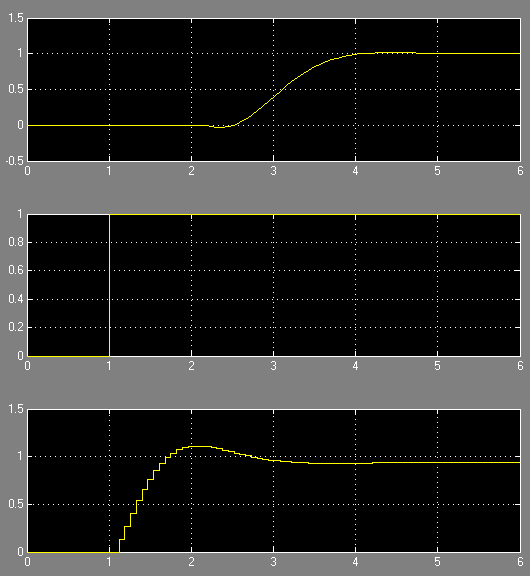
\includegraphics[width=0.8\textwidth]{Imagens/q13.png}
        \caption{Estrutura do Preditor de Smith.}
    \end{figure}
    
    \textbf{Resultado:} O desempenho do controlador é restaurado, mesmo com o grande atraso. A técnica é essencial para sistemas com atrasos de transporte significativos.
\end{frame}

\begin{frame}{Conclusões: A Moral da História}
    \huge \textbf{O que aprendemos?}
    
    \vspace{1.5em}
    
    \begin{itemize}
        \item<1-> \large \textbf{Não existe "bala de prata".} A escolha do controlador é um balanço entre desempenho, complexidade e custo.
        \begin{itemize}
            \item \textbf{PI:} Simples, robusto, mas limitado.
            \item \textbf{LR + FF:} Desempenho superior, mas mais complexo e caro (requer sensor extra).
            \item \textbf{Preditor de Smith:} Essencial para atrasos, mas sensível a erros de modelagem.
        \end{itemize}
        
        \item<2-> \large \textbf{Conhecer o inimigo é fundamental.} Medir e antecipar a perturbação (Feedforward) transforma o desempenho do controle.
        
        \item<3-> \large \textbf{O mundo real tem atrasos.} Ignorá-los pode levar à instabilidade. Técnicas específicas são necessárias para garantir um controle eficaz.
    \end{itemize}
\end{frame}

\begin{frame}
    \centering
    \Huge\bfseries Perguntas?
    \vspace{2em}
    
    \large Obrigado!
\end{frame}

\end{document}
